\chapter{Proposta}\label{cap3}


Essa seção apresenta as etapas de desenvolvimento do sistema, bem como o seu funcionamento geral, desde a preparação dos documentos até a entrega dos históricos de ocorrência ao usuário. Inicialmente serão descritos a seleção e pré-processamento. Em seguida, será relatado como as técnicas de mineração de texto e resgate de informação são utilizadas nesse trabalho.

O objetivo do sistema é permitir ao usuário consultar uma coleção de documentos de reuniões a fim de obter todo o histórico de ocorrências de um determinado tema pesquisado, podendo identificar nos documentos onde o tema foi mencionado como informe ou onde houve uma decisão sobre o tema. Para isso, o sistema é divido em dois módulos principais: Módulo de preparação e manutenção e Módulo de consulta.

O módulo de preparação e manutenção recebe uma coleção de documentos e produz uma estrutura de dados interna, que é utilizada pelo módulo de consulta, que por sua vez, é responsável por receber a intensão usuário, proceder a busca na estrutura de dados interna e retornar os trechos associados com a intensão do usuário, tanto quanto ao assunto como no tipo de ocorrência. A Figura \ref{fig:visao-geral} mostra a visão geral do sistema com suas principais entradas e saídas. 


  %--- Figura Visão Geral ---
  \begin{figure}[!h]
	  \centering
	  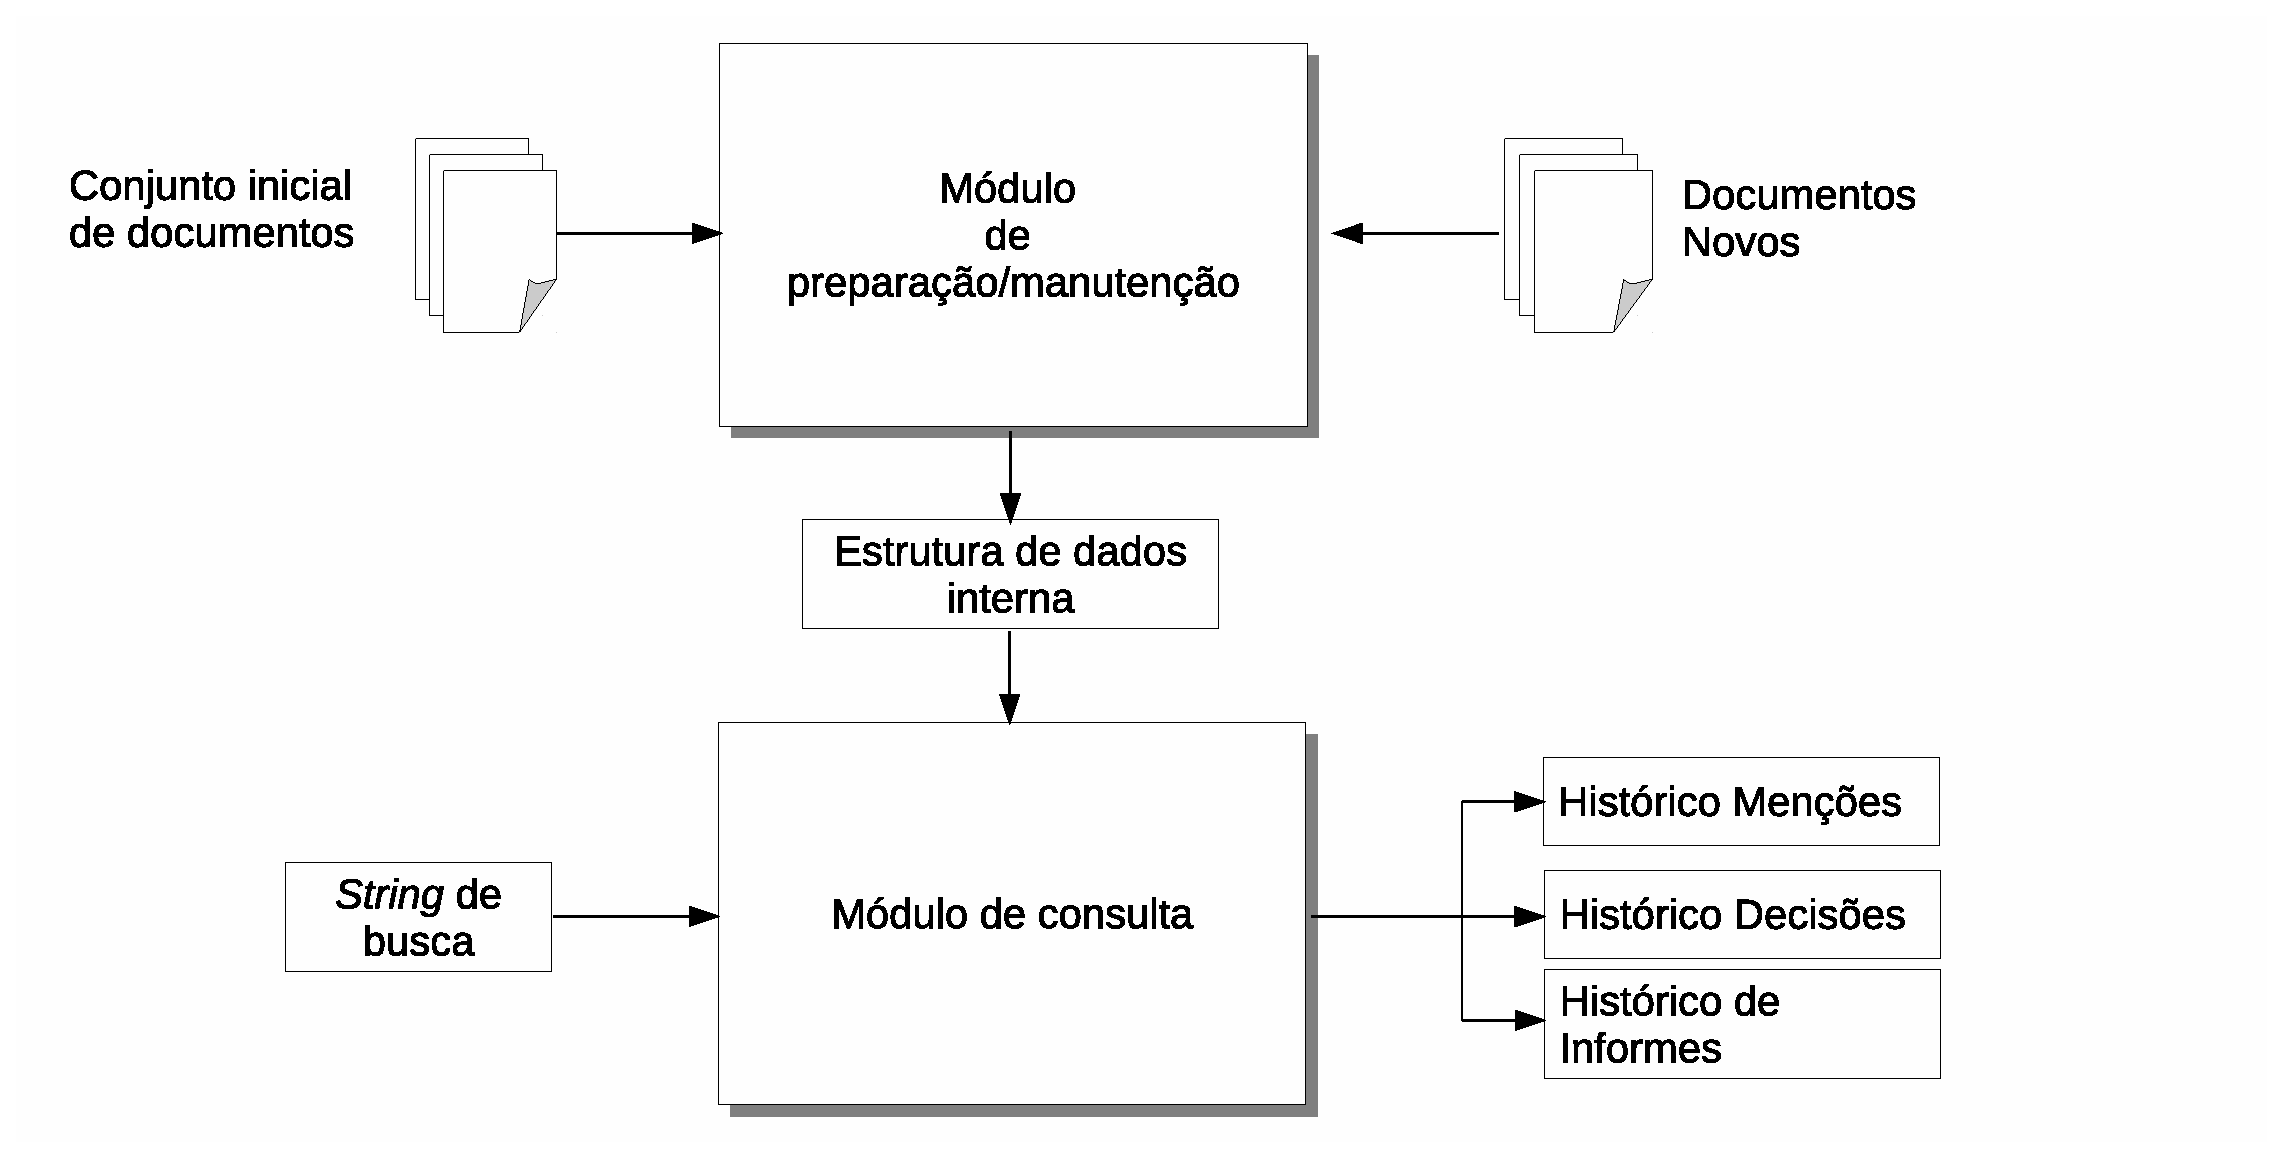
\includegraphics[width=0.69\paperwidth]{conteudo/capitulos/figs/visao-geral-3.eps}
	  \caption{Visão geral do sistema}
	  \label{fig:visao-geral}
  \end{figure}






\section{Módulo de preparação e manutenção}

O módulo de preparação e manutenção tem como funções principais dividir cada ata em em segmentos de texto que contêm um assunto predominante, e descrevê-los por meio de técnicas de extração tópicos e classificação. Além disso, produz uma estrutura de dados que registra quais assuntos foram tratados na reunião, bem como o trecho do documento onde é discutido.


\subsection{Preparação dos documentos}

As atas são normalmente armazenadas em arquivos do tipo \textit{pdf}, \textit{doc}, \textit{docx} ou \textit{odt} que normalmente possuem formato binário.
O texto deve ser preparado para os métodos de MT e RI. Inicialmente, o texto puro é extraído e passa por processos de transformação conforme apresentados a seguir.


\begin{enumerate}

%  Cabeçalhos e rodapés
\item Remoção de cabeçalhos e rodapés: as atas contém trechos que podem ser considerados pouco informativos e descartados durante o pré-processamento, como cabeçalhos e rodapés que se misturam aos tópicos tratados na reunião, podendo ser  inseridos no meio de um tópico prejudicando tanto os algoritmos de MT e RI, quanto a leitura do texto pelo usuário.

%  Identificação de sentenças
\item Identificação de finais sentenças: devido ao estilo de pontuação desses documentos, como encerrar sentenças usando um \textit{";"} e inserção de linhas extras, foram usadas as regras especiais para identificação de finais de sentença. Cada final de sentença é identificado e marcado com uma \textit{string} especial.%, esse processo é melhor descrito na Subseção~\ref{subsec:indentificacaosentencas}. % Os detalhes sobre essas regras estão disponíveis para consulta em \urlsoftwares.


% \item Segmentação


%  Remoção de termos
\item Redução de termos: eliminou-se as \textit{stop words} por meio de uma lista de 438 palavras. Além disso, eliminou-se a acentuação, sinais de pontuação, numerais e todos os \textit{tokens} menores que três caracteres. 

%  Stemming
\item \textit{Stemming}: extraiu-se o radical de cada palavra. Para isso, as letras foram convertidas em caixa baixa e aplicou-se o algoritmo \textit{Orengo}%\footnote{\urlorengo} 
	para remoção de sufixos.

\end{enumerate}
	

A Figura~\ref{fig:exemplopreprocessamento} mostra a etapa de preparação de um documento em português.
	


  \begin{figure}
	\centering
	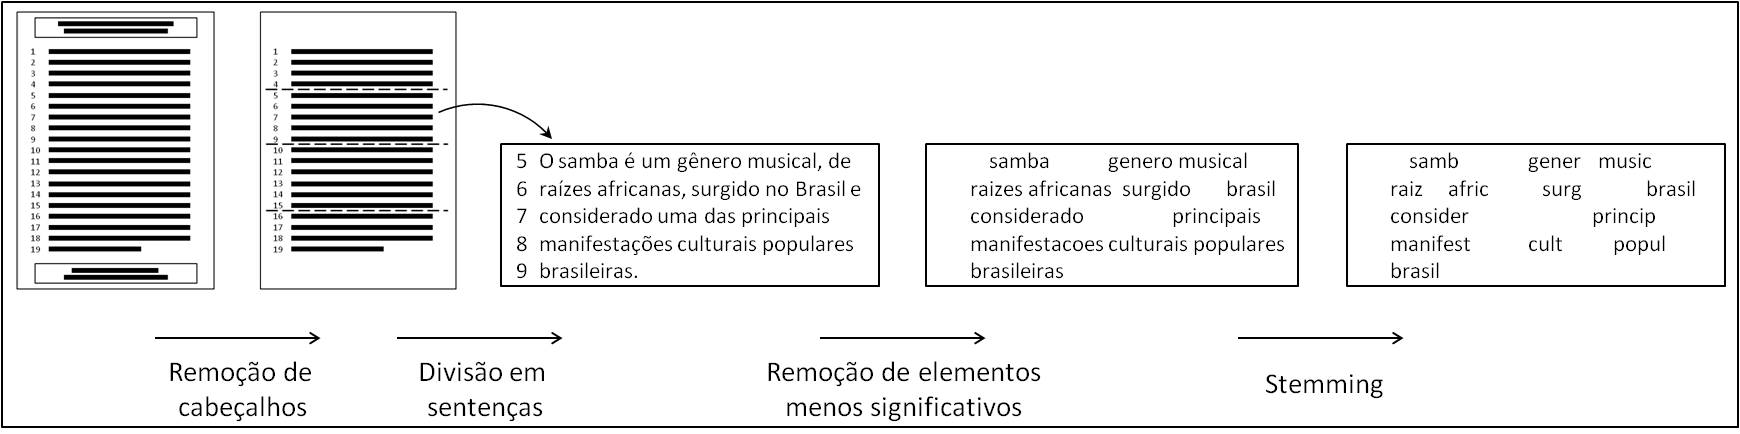
\includegraphics[width=1\textwidth]{conteudo/capitulos/figs/pre-processamento.jpg}
	\caption{Exemplo de pré-processamento.}
	\label{fig:exemplopreprocessamento}
  \end{figure}

% -< Ao final .....


\subsubsection{Segmentação}


Como já mencionado, uma ata registra a sucessão de assuntos discutidos em uma reunião, porém apresenta-se com poucas quebras de parágrafo e sem marcações de estrutura, como capítulos, seções ou quaisquer indicações sobre o assunto do texto. Portanto, faz-se necessário descobrir quando há uma mudança de assunto no texto da ata. Para essa tarefa, as técnicas de segmentação de texto recebem uma lista de sentenças, da qual considera cada ponto entre duas sentenças como candidato a limite, ou seja, um ponto onde há transição entre assuntos. 


Entre os principais trabalhos da literatura podemos citar o  \textit{TextTiling} %~\cite{Hearst1994} 
e o \textit{C99}%~\cite{Choi2000}
.
% 
% ------   TextTiling
O \textit{TextTiling} é um algoritmo baseado em janelas deslizantes, em  que, para cada candidato a limite, analisa-se o texto circundante. Um limite ou quebra de segmento é identificado sempre que a similaridade estiver abaixo de um limiar. Possui baixa complexidade computacional e acurácia semelhante a algoritmos mais complexos baseados em matrizes de similaridade como o \textit(C99).

Para cada posição candidata o \textit{TextTiling} constrói 2 blocos, um contendo sentenças que a precedem e outro com as que a sucedem. O tamanho desses blocos é um parâmetro a ser fornecido ao algoritmo e determina o tamanho mínimo de um segmento.

% ------   C99
O \textit{C99} usa matrizes de \textit{rakings} de similaridades e técnicas de \textit{clustering} para encontrar os limites entre os segmentos. Oferece resultados melhores que algoritmos baseados em janelas deslizantes ao custo de maior complexidade computacional.

Inicialmente é construída uma matriz que contém as similaridades de todas as unidades de texto. Em seguida, essa é transformada substituindo-se cada elemento da matriz original pelo número de elementos vizinhos com similaridade inferior.  Finalmente, utiliza um método de \textit{clustering} % baseado no algoritmo de maximização de Reynar % ~\cite{Reynar1998} 
para identificar os limites entre os segmentos. 



% ----------------------------------------------------------------------------- 


% usando um conjunto de documentos e uma segmentação manual fornecida por participantes das reuniões. 


% explicar o qe o segmentador faz --> encontrar limites



\subsubsection{Avaliação dos Segmentadores}


%  Critérios de avaliação

Para que se possa avaliar um segmentador automático de textos é preciso uma referência, isto é, um texto com os limites entre os segmentos conhecidos. Essa referência, deve ser confiável, sendo uma segmentação legítima que é capaz de dividir o texto em porções relativamente independentes, ou seja, uma segmentação ideal.

Para este trabalho, um bom método de segmentação é aquele cujo resultado melhor se aproxima de uma segmentação manual, sem a obrigatoriedade de estar perfeitamente alinhado com tal. Ou seja, visto o contexto das atas de reunião, e a subjetividade da tarefa, não é necessário que os limites entre os segmentos (real e hipótese) sejam idênticos, mas que se assemelhem em localização e quantidade.

Os algoritmos foram comparados com a segmentação fornecida pelos participantes das reuniões e calculou-se as medidas mais aplicadas à segmentação textual, P$_k$ e \textit{WindowDiff}. Além dessas, computou-se também as medidas tradicionais acurácia, precisão, revocação e $F^1$ para comparação com outros trabalhos que as utilizam.

O algoritmo \textit{C99} obteve melhor desempenho em acurácia, precisão, $F^1$, $P_k$ e \textit{WindowDiff}, enquanto o \textit{TextTiling} obteve o melhor desempenho em revocação como pode ser visto na Tabela~\ref{tab:configfinal}. 


\begin{table}[!h]
	\centering

	\begin{tabular}{|l|l|c|c|c|c|c|} \hline
		\textbf{Algoritmo} & 
		\textbf{Medida} & 
		\textbf{Média}\\	\hline

	\textit{C99} & P$_k$			   & 0,116 \\ \hline
	\textit{C99} & \textit{WindowDiff} & 0,390 \\ \hline
	\textit{C99} & Acurácia			   & 0,609 \\ \hline
	\textit{C99} & Precisão			   & 0,720 \\ \hline
	\textit{C99} & F$^1$			   & 0,655 \\ \hline
	\textit{TextTiling} &	Revocação  & 0,917 \\ \hline

	\end{tabular}
	
	\caption{Melhores resultados obtidos.}
	\label{tab:configfinal}
\end{table}





%  we have a winner
Verificou-se que, de maneira geral, o algoritmo \textit{C99} apresenta melhores resultados em relação ao \textit{TextTiling}, contudo, testes estatísticos realizados indicaram que não houve diferença significativa entre os métodos. Nesse trabalho, escolheu-se o algoritmo \textit{C99} por apresentar resultados satisfatórios e ligeira superioridade em relação ao \textit{TextTiling}. 



%  ==========   ==========   ==========   ==========   ==========   



% cada segmento é um documento
Após a identificação dos segmentos, o algoritmo retorna uma lista onde cada elemento é um texto com um assunto predominante e será a partir de disso considerado um documento.

% -? Medidas

% -- como ele faz?





\subsection{Representação Computacional}

As etapas anteriores produzem fragmentos de documentos onde o texto esta em um estágio de processamento inicial, com menos atributos que as versões originais, onde cada fragmento está associado a um tema, porém, ainda não estruturado. Ocorre que as técnicas de mineração de texto exigem uma representação estruturada dos textos. % conforme será visto na Seção~\ref{subsection:RepTextos}.

Uma das formas mais comuns é a representação no formato matricial conhecida como Modelo Espaço Vetorial (\textit{Vectorial Space Model} - VSM)~\cite{Rezende2003}, onde os documentos são representados como vetores em um espaço Euclidiano $t$-dimensional em que cada termo extraído da coleção é representado por um dimensão. Assim, cada componente de um vetor expressa a relação entre os documentos e as palavras. Essa estrutura é conhecida como \textit{document-term matrix} ou matriz documento-termo.

A forma adotada nesse trabalho é a \textit{Bag Of Words} a qual sintetiza a base de documentos em um contêiner de palavras, ignorando a ordem em que ocorrem, bem como pontuações e outros detalhes, preservando apenas o peso de determinada palavra nos documentos. É uma simplificação de toda diversidade de informações contidas na base de documentos sem o propósito de ser uma representação fiel do documento, mas oferecer a relação entre as palavras e os documentos a qual é suficiente para a maioria dos métodos de aprendizado de máquina.%~\cite{Rezende2003}. 

% será empregada por ser a mais utilizada e referenciada na literatura e por sua simplicidade e qualidade dos resultados que são obtidos. 





\subsection{Extração de Tópicos / Classificação de Textos}

% a tarefa é identificar qual assunto está presente em cada trecho e qual é o tipo de ocorrência.



\section{Módulo Consulta}

Uma vez que a estrutura de dados interna contem os assuntos abordados na coleção de documentos, o tipo de ocorrência para cada assunto e o trecho onde se encontram, caberá ao módulo de consulta receber a \textit{string} de consulta do usuário, resgatar os dados desejados e apresentá-los em ordem cronológica, dando condições para o usuário acessar os segmentos encontrados bem como os documentos originais.

\subsection{Seleção dos tópicos}

\subsection{Visualização}

O usuário final precisa de uma interface adequada para visualizar os resultados da busca considerando-se a relevância dos tópicos selecionados e a sequência cronológica.

Uma boa apresentação deve permitir ao usuário identificar a relevância os resultados e ser relativante independente para compreensão do conteúdo, evitando a leitura do texto completo. Ou seja, o texto de cada tópico apresentado deve ser suficiente para compreensão do assunto mencionado, sem necessidade de visualizar o documento original.

As informações apresentadas, incluem dados obtidos do documento como o nome do arquivo e data do original e o texto onde o assunto é mencionado. Além disso, apresenta-se as informação extraídas pelas técnicas de mineração de texto como os descritores e rótulos.

% o sistema traz vários resultados para uma consulta, alguns mais relevantes que outros. Para cada resultado (que podem tratar de coisas diferentes) o sistema apresenta um histórico de menções para aquele assunto;

Para cada busca, é retornada uma lista de resultados ordenados pela relevância com a \textit{string} de entrada, sendo cada item referente a uma menção a um assunto. Um tópico é abordado em diferentes momentos e registrado em atas distintas, onde cada menção é um resultado a ser apresentado. 

Como parte da proposta, o sistema apresenta cada resultado dentro de um histórico de menções. Para isso, abaixo do texto é exibida uma linha com links para os resultados que compartilham o mesmo tópico ordenados por data. Os links, ao ser acionado, direciona para o resultado que aponta, além disso, quando o cursor do mouse está sobre o link, é apresentado um pre-visualização do texto. Dessa forma o usuário tem acesso uma interface que lhe fornece uma visão temporal das menções.

% Uma vez que um item faz menção a um tópico específico, 


% um histórico de menções para o assunto pesquisado.
% O sistema também apresenta junto com cada resultado, 


\section{Estudo de caso}
% -- qual o ganho em relação a um sitema de busca por palavras-chave? 


\section{Avaliação}

